\emph{\underline{Objetivo:}}\bigskip \\ Visualizaci'on por la pantalla del PDA del expediente de un paciente del hospital.\bigskip \\ \emph{\underline{Entradas:}}
\begin{itemize}
\item Nombre del paciente del que queremos consultar el expediente.
\end{itemize}

\emph{\underline{Precondiciones:}}\bigskip \\ El propietario del expediente que queremos visualizar debe ser un paciente registrado en la base de datos del hospital.\bigskip \\ \emph{\underline{Salidas:}}\bigskip \\ En caso de \'exito (el nombre paciente se encuentra en la base de datos del hospital): 
\begin{itemize}
	\item Se muestra en la pantalla del PDA el expediente del paciente solicitado.
\end{itemize}

En caso de fallo (el nombre paciente no se encuentra en la base de datos del hospital): 
\begin{itemize}
	\item Se informa al usuario de la imposibilidad de visualizar la informaci'on solicitada.
	\item Se vuelve al men'u principal.
\end{itemize}

\emph{\underline{Postcondici\'on si \'exito (el nombre paciente se encuentra en la base de datos del hospital):}}\bigskip \\ Se muestra el expediente del paciente solicitado en la pantalla del PDA.\bigskip \\ \emph{\underline{Postcondici\'on si fallo (el nombre paciente no se encuentra en la base de datos del hospital):}}\bigskip \\ Se informa al usuario de la imposibilidad de visualizar los datos solicitados y se vuelve al men'u principal.\bigskip \\ \emph{\underline{Actores: }}
\begin{itemize}
	\item Usuario con PDA.
	\item Servidor del hospital.
	\item PDA.
\end{itemize}

\emph{\underline{Secuencia normal:}}
\begin{enumerate}
	\item El usuario solicita al servidor la consulta del expediente de un paciente del hospital desde su PDA.
	\item El servidor busca en su base de datos el expediente del paciente solicitado. En caso de que la b\'usqueda tenga \'exito pasar a 3, en caso contrario pasar a E1.
	\item Se hace una lectura del expediente solicitado y se env'ia al PDA, mostr'andose por pantalla.
	\item Volvemos al men'u principal.
\end{enumerate}

\emph{\underline{Secuencias alternativas:}}\bigskip \\ E1.- Se informa al usuario del error en la consulta y se vuelve al men'u principal.\bigskip \\ Para ilustrar mejor est'a secuencia de acciones, incluimos el diagrama de secuencia de este caso de uso (Figura \ref{fig:consulta_expediente})

\begin{figure*}[h!]
	\begin{center}
        		%\framebox{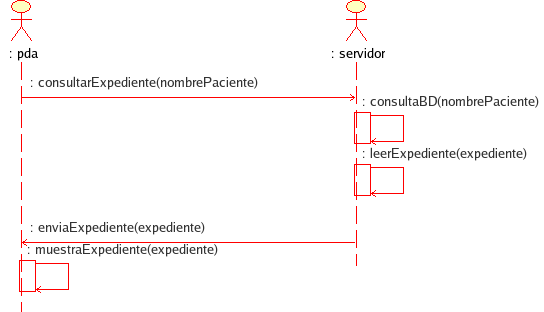
\includegraphics[scale=0.4]{consultar_expediente.png}}
		\framebox{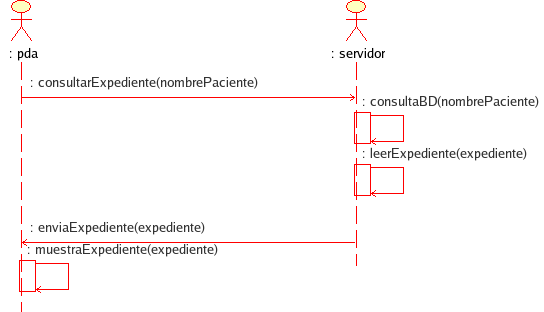
\includegraphics[scale=0.6]{consultar_expediente.png}}
     	\end{center}
    	\caption{Diagrama de secuencia de consultar expediente}\label{fig:consulta_expediente}
\end{figure*}
\pagebreak
\newpage 